\documentclass[12pt]{article}

\usepackage[letterpaper,margin=1in]{geometry}
\usepackage[T1]{fontenc}
\usepackage{lmodern}
\usepackage{microtype}
\usepackage{amsmath,amssymb}
\usepackage{graphicx}
\usepackage{booktabs}
\usepackage[font=small,labelfont=bf,skip=4pt]{caption}
\usepackage[round,authoryear]{natbib}
\usepackage[hidelinks]{hyperref}
\usepackage[capitalise,noabbrev]{cleveref}
\usepackage{enumitem}
\usepackage{float}

\setlength{\parskip}{0.35em}
\setlength{\textfloatsep}{12pt plus 2pt minus 2pt}
\setlist{itemsep=1pt,topsep=3pt}
\graphicspath{{figures/}}

\newcommand{\Count}{\textsc{Count}}
\newcommand{\Jac}{\textsc{Jaccard}}
\newcommand{\Wtd}{\textsc{Weighted}}
\newcommand{\SVD}{\textsc{SVD}}

\title{\vspace{-1.6em}From Purchases to Communities:\\[2pt]
\large How User Activity Shapes Product Networks Built from Purchase Data}
\author{Tong Zhou \and Sia Xie \and Yilin Jiang \and Mingjiao Diao}
\date{STAT 236, Fall 2026}

\begin{document}
\maketitle
\vspace{-1.2em}

\begin{abstract}
\noindent
Product networks built from purchase data link two products whenever the same customer buys both. A customer who buys $d$ products contributes $d(d-1)/2$ links, so very active customers can dominate the network, and a common response is to downweight them. We ask when this helps. In a simulation with known product categories, we compare raw co-purchase counts, Jaccard similarity, inverse-activity weighting, and a normalized SVD of the user--product matrix while varying how unevenly activity is spread and whether active users have category preferences. When active users focus on one category they carry most of the signal, and downweighting them is costly: with the most concentrated activity, weighting raises the misclustering rate from 13\% to 49\%. When active users buy indiscriminately, our main design leaves too little signal for any method to recover the categories. Post hoc experiments that hold informative purchases fixed show the opposite effect: added preference-free heavy buyers drive raw counts to chance while weighting stays near its baseline. Activity is not a proxy for noise; whether to downweight it depends on what active users buy.
\end{abstract}

% =====================================================================
\section{Introduction}

Purchase records form a bipartite network between users and products. A standard way to analyse such data is to \emph{project} it onto the products, connecting two products when they share buyers, and then to cluster the resulting network \citep{vonluxburg2007,ke2026}. The clusters describe groups of products that tend to be bought by the same people.

The projection has a well-known weakness: a user who buys $d$ distinct products creates $d(d-1)/2$ product pairs, so a handful of heavy buyers can supply most of the edge weight. The usual remedy, going back to the collaboration networks of \citet{newman2001}, is to give each user's pairs weight $1/(d-1)$, which makes a user's total contribution grow only linearly.

Whether this is a good idea depends on what active users buy, which the weighting ignores (\cref{fig:schematic}). If a heavy buyer spreads purchases across categories, most of their links cross category boundaries and downweighting removes noise; if the same buyer concentrated on one category, downweighting would discard the strongest evidence in the data. We study this tension with three questions:
\begin{enumerate}[label=\textbf{Q\arabic*.},leftmargin=2.6em]
  \item How do activity heterogeneity and the breadth of active users' preferences interact with the choice of projection weights?
  \item When does inverse-activity weighting improve on raw counts and Jaccard similarity?
  \item How do the projections compare with a normalized SVD applied directly to the user--product matrix?
\end{enumerate}

\begin{figure}[t]
  \centering
  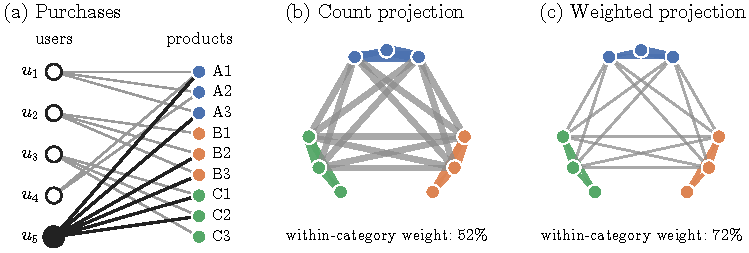
\includegraphics[width=\textwidth]{fig1_schematic}
  \caption{A toy example. Users $u_1$--$u_4$ buy within a single category; $u_5$ buys six products across all three. (b)~Under counts, every pair created by $u_5$ has full weight and cross-category edges (grey) dominate. (c)~Inverse-activity weighting gives each of $u_5$'s pairs weight $1/5$, and the within-category share of edge weight rises from 52\% to 72\%. If $u_5$ instead bought six products from one category, the same weighting would shrink useful edges.}
  \label{fig:schematic}
\end{figure}

We answer these questions with a simulation in which product categories are known, total purchases are matched across conditions, and expected edge weights can be computed exactly; all methods are applied to the same data sets.

\paragraph{Related work.} Our $1/(d-1)$ weight follows \citet{newman2001}. \citet{zhou2007} also discount active users in a resource-allocation projection for recommendation. The SVD baseline is motivated by bipartite spectral co-clustering \citep{dhillon2001} and its extension to directed graphs \citep{rohe2016}, though we do not implement either algorithm exactly.

% =====================================================================
\section{Model and methods}

\subsection{A simple purchase model}

Let $B\in\{0,1\}^{n\times p}$ record purchases, with $B_{ui}=1$ if user $u$ bought product $i$. We use $n=1{,}000$ users and $p=300$ products divided into $K=3$ categories of $s=p/K=100$ products. Each user has a preferred category, drawn uniformly at random, and buys $d_u$ distinct products one at a time without replacement. At each draw, a remaining product in the preferred category has weight $r_u\ge 1$ and every other product has weight 1. With $r_u=2$, about half of a user's purchases fall in the preferred category; with $r_u=1$ the user has no preference at all.

\subsection{Three product networks}

Let $S_{ij}=\sum_u B_{ui}B_{uj}$ be the number of shared buyers of products $i\ne j$ and $b_i=\sum_u B_{ui}$ the number of buyers of $i$. We compare
\begin{align*}
  W^{\text{count}}_{ij} &= S_{ij}, &
  W^{\text{jac}}_{ij} &= \frac{S_{ij}}{b_i+b_j-S_{ij}}, &
  W^{\text{wtd}}_{ij} &= \sum_{u:\,d_u\ge 2}\frac{B_{ui}B_{uj}}{d_u-1}.
\end{align*}
All diagonals are set to zero and no edges are thresholded. For each network $W$ with degree matrix $D$, we take the eigenvectors of $D^{-1/2}WD^{-1/2}$ belonging to the $K$ largest eigenvalues, normalize each row of the resulting embedding, and run $k$-means with 20 random starts.

As a fourth method we skip the projection. We form $M=D_u^{-1/2}BD_p^{-1/2}$, where $D_u$ and $D_p$ hold user and product degrees, and cluster the products using the top $K$ right singular vectors of $M$, with the same row normalization and $k$-means step. Since
\begin{equation}
  M^\top M = D_p^{-1/2}\,B^\top D_u^{-1} B\, D_p^{-1/2},
  \label{eq:svd}
\end{equation}
this baseline is itself a projection that weights each user by $1/d_u$, close to the $1/(d_u-1)$ of \Wtd. The main differences are that it keeps the diagonal of $M^\top M$ and that users with a single purchase still enter it.

\subsection{Expected edge weights and user influence}

Because products within a category are exchangeable, the probability that user $u$ buys a particular pair of distinct products depends only on whether the two products share a category. Writing $C_{uk}$ for the number of products $u$ buys from category $k$,
\[
  q^{\text{same}}_u=\frac{\mathbb{E}[C_{uk}(C_{uk}-1)]}{s(s-1)},\qquad
  q^{\text{diff}}_u=\frac{\mathbb{E}[C_{uk}C_{ul}]}{s^2}\quad(k\ne l).
\]
Summing $q_u$ over users gives the expected \Count{} weight of a within- or between-category pair; dividing each term by $d_u-1$ gives the \Wtd{} expectation. We compute the required moments exactly with a short dynamic program over the sequential sampling scheme (\cref{app:recurrence}). For \Jac{} we use the ratio of expected shared buyers to expected union size, an approximation that agrees with the simulated means to within 0.23\% in every condition (\cref{app:theory}).

Two facts follow directly. A user with $r_u=1$ has $q^{\text{same}}_u=q^{\text{diff}}_u$ and adds no expected within-minus-between contrast, and a user with $d_u\ge 2$ contributes total weight $d_u(d_u-1)/2$ under \Count{} but only $d_u/2$ under \Wtd. \Cref{fig:influence}(b) shows what this means in our design. With focused users and the most concentrated activity, the top 20\% of users supply 99.6\% of the expected \Count{} contrast; weighting reduces their share to 84.0\%. Shares measured in the simulated data agree to within 0.2 percentage points.

\begin{figure}[t]
  \centering
  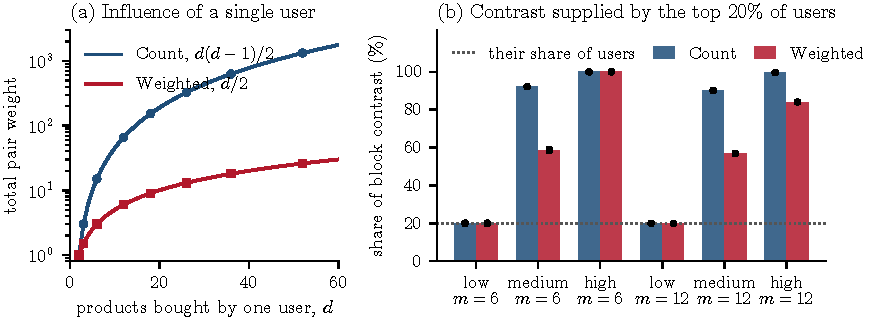
\includegraphics[width=\textwidth]{fig2_influence}
  \caption{(a) Total pair weight contributed by one user who buys $d$ products; markers show the purchase counts used in our design. (b) Share of the expected within-minus-between contrast supplied by the 20\% most active users when all users are focused ($r=2$). Bars are exact expectations; black points are means over 100 simulated data sets with 95\% intervals. Under low heterogeneity the ``active'' 20\% are a random subset of equally active users.}
  \label{fig:influence}
\end{figure}

% =====================================================================
\section{Experimental design}

We vary three factors (\cref{tab:design}). \emph{Density} sets the mean number of purchases per user, $m\in\{6,12\}$. \emph{Activity heterogeneity} determines how those purchases are spread: equally, or with 20\% of users buying three or more times the mean. Total purchases are identical across heterogeneity levels, so only their concentration changes. \emph{Preference breadth} is either \emph{focused}, where every user has $r_u=2$, or \emph{broad active}, where the 20\% most active users have $r_u=1$ and the rest keep $r_u=2$. Activity is assigned independently of the preferred category. Crossing the factors gives 12 conditions, each with 100 independent data sets.

\begin{table}[t]
  \centering
  \caption{Purchase counts per user. Within each density, total purchases are the same in every column.}
  \label{tab:design}
  \begin{tabular}{@{}lccc@{}}
    \toprule
    Mean purchases $m$ & Low heterogeneity & Medium heterogeneity & High heterogeneity \\
    \midrule
    6  & all users buy 6  & 80\% buy 3, 20\% buy 18 & 80\% buy 1, 20\% buy 26 \\
    12 & all users buy 12 & 80\% buy 6, 20\% buy 36 & 80\% buy 2, 20\% buy 52 \\
    \bottomrule
  \end{tabular}
\end{table}

The settings were fixed after a pilot of 10 data sets per condition. Following our proposal, we required at least two conditions with a median error between 5\% and 40\% for some method; four met it at $r=2$, so we kept the initial design, without regard to which method performed best, and ran the main experiment with fresh seeds.

Our primary measure is the \emph{misclustering rate}: the fraction of the 300 products assigned to the wrong category after the best matching of cluster labels to categories. To judge how far a method is from chance, we permute the true labels and recompute the matched error; across all conditions this random-label reference lies between 62.9\% and 63.5\%. All intervals are 95\% intervals for a mean over 100 independent data sets. Method comparisons are paired within data sets and are not adjusted for multiple comparisons.

% =====================================================================
\section{Results}

\subsection{Recovery across the design}

\Cref{fig:recovery} summarizes the main experiment. When active users are focused (left column), concentrating activity helps \Count{} and \Jac{} but hurts \Wtd{} and \SVD. At $m=12$, \Count{} error falls from 35.5\% under equal activity to 22.4\% and then 13.0\% as activity becomes more concentrated, while \Wtd{} rises from 35.3\% to 39.1\% and 48.6\%. Heavy buyers who stay within their category are the most informative users in the data, and the count projection lets them speak loudest.

At $m=6$ the pattern is weaker. At high heterogeneity \Count{} and \Wtd{} coincide (41.3\% and 41.2\%): the 80\% of users with one purchase contribute no pairs, so every contributing user buys 26 products and the two weightings differ by a constant.

When the active users are broad (right column), recovery is poor under medium and high heterogeneity: every method is within about three points of the random-label reference. With equal activity it is better (48.5\% at $m=12$) because the broad users are no more active than anyone else.

\begin{figure}[t]
  \centering
  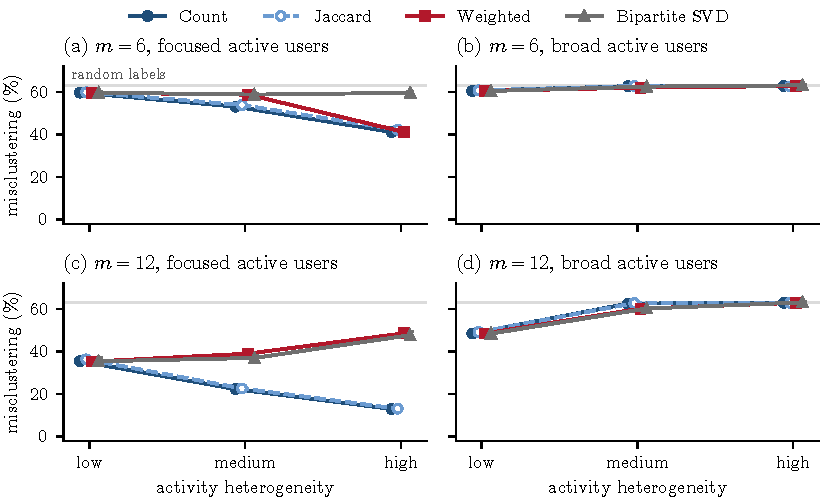
\includegraphics[width=\textwidth]{fig3_recovery}
  \caption{Mean misclustering rate in the main experiment ($r=2$). Each point averages 100 data sets; error bars are 95\% intervals and are often smaller than the markers. The grey band marks the random-label reference.}
  \label{fig:recovery}
\end{figure}

\subsection{The paired effect of weighting}

Comparing \Count{} and \Wtd{} on the same data sets isolates the effect of weighting (all 12 paired differences are shown in \cref{fig:paired}). With focused active users, weighting costs 16.7 percentage points at $m=12$ and medium heterogeneity (95\% interval 15.2 to 18.2) and 35.6 points at high heterogeneity (34.1 to 37.0). Its only clear gains occur with broad active users at medium heterogeneity, 2.4 points at $m=12$ (1.8 to 3.0) and 0.7 points at $m=6$, and both leave the error close to chance. Under equal activity the two networks are proportional, so their normalized matrices are identical and the small differences come from $k$-means initialization.

Why does weighting not rescue the broad-active conditions? At $m=6$ and high heterogeneity, the 800 users with preferences buy one product each and create no pairs, while the 200 heavy buyers have no preference. The expected block contrast is exactly zero under every projection, and no reweighting can create signal that is not there. At $m=12$, the focused users buy two products each and the broad users 52, so a broad user contributes 1{,}326 pairs under \Count{} and 26 under \Wtd, against one for a focused user. Weighting lowers the broad users' share of pair weight from 99.7\% to 86.7\%, but they still dominate. Because total purchases are matched, making active users broad also takes purchases away from informative users, a confound we remove in \cref{sec:posthoc}.

\subsection{Jaccard and the bipartite SVD}

\Count{} and \Jac{} are nearly interchangeable here: their edge weights have a mean Spearman correlation of 0.97 and their mean errors never differ by more than 1.0 point, although their partitions still differ (mean adjusted Rand index 0.70). This is expected when all products in a category are equally popular.

The bipartite \SVD{} tracks \Wtd{}, as \eqref{eq:svd} predicts, and offers no general advantage: with focused users at $m=12$ and high heterogeneity its error exceeds that of \Count{} by 34.7 points (33.2 to 36.2), and at $m=6$ it trails both projections (59.7\% against 41\%).

% =====================================================================
\section{Post hoc analyses}
\label{sec:posthoc}

The main experiment leaves Q2 only half answered: weighting clearly hurts when active users are focused, but we cannot tell whether it would help against broad active users if enough signal remained. After reviewing the main results, we designed three further analyses and recorded their settings before running them. They are post hoc and leave the main design and results unchanged; each condition uses 100 fresh data sets (4{,}200 in total).

\paragraph{Stronger preferences.} We reran the full design with $r=3$ and with $r=4$, the upper value listed in our proposal (\cref{fig:strength}; complete results in \cref{app:tables}). With broad active users at $m=12$ and medium heterogeneity, the methods now separate. \Count{} and \Jac{} stay at chance, while \Wtd{} falls to 34.8\% at $r=3$ and 9.6\% at $r=4$. The paired advantage of weighting is 27.7 points (26.1 to 29.3) and 51.5 points (50.8 to 52.2). In the focused conditions, stronger preferences make recovery easy for every method, so the cost of weighting shrinks; at $r=4$ all three projections stay below 5.4\% error. At high heterogeneity the broad-active conditions remain at chance for the reason given above.

\begin{figure}[t]
  \centering
  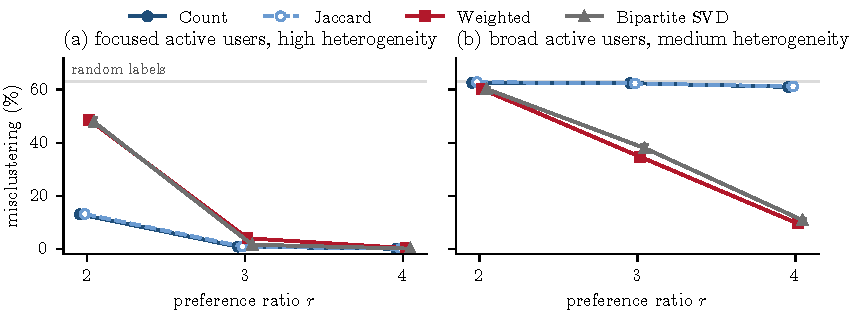
\includegraphics[width=\textwidth]{fig5_strength}
  \caption{Misclustering rate as preference strength increases, at $m=12$. Values at $r=2$ are from the main experiment; $r=3$ and $r=4$ are post hoc. Error bars are 95\% intervals.}
  \label{fig:strength}
\end{figure}

\paragraph{Holding the informative purchases fixed.} To isolate the effect of noisy heavy buyers, we fixed 1{,}000 informative users in one of two settings ($m=12$, $r=2$ or $m=6$, $r=3$), then added $A=50$ or $200$ users with no preference who each buy $D$ products, with $D/m\in\{1,2,4,8\}$. Within each replicate the informative purchases are identical across conditions. Unlike the main design, total purchases now grow as background is added.

\begin{figure}[t]
  \centering
  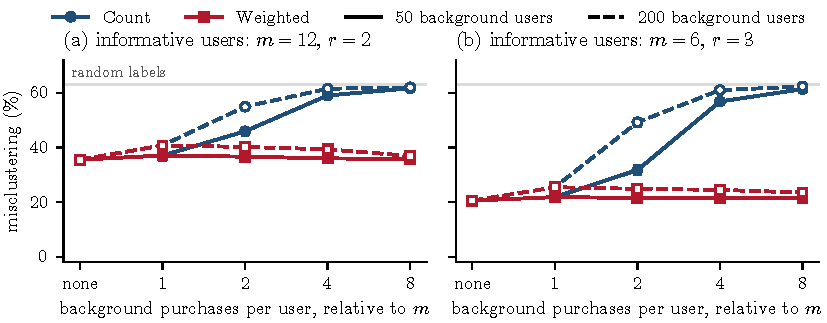
\includegraphics[width=\textwidth]{fig6_separation}
  \caption{Adding preference-free users to 1{,}000 fixed informative users: solid lines add 50, dashed lines 200. \Jac{} behaves like \Count{} and \SVD{} like \Wtd{} (\cref{app:tables}).}
  \label{fig:separation}
\end{figure}

The result is clear (\cref{fig:separation}). In the first setting, 50 background users buying $4m=48$ products each push \Count{} from 35.5\% to 59.1\%, whereas \Wtd{} stays at 36.0\%; the paired difference is 23.0 points (21.4 to 24.7). In the second setting the difference at $D=4m$ is 35.2 points (33.9 to 36.5). When $D=m$ the background users are no more active than anyone else, weighting cannot single them out, and the two methods give identical results. Weighting does not make recovery immune to background: with 200 background users, \Wtd{} also loses a few points.

\paragraph{Why the SVD fails at $m=6$.} Users with one purchase contribute nothing to any projection but still enter the SVD through $D_u$, $D_p$, and the diagonal of $M^\top M$. Rerunning the SVD on the recorded data sets without them (after checking that the original errors are reproduced exactly) brings it in line with \Count{} at $m=6$; at $m=12$, where no user buys a single product, nothing changes (\cref{tab:ablation}).

\begin{table}[t]
  \centering
  \caption{SVD with and without single-purchase users (focused users, high heterogeneity). Mean error (\%) over 100 recorded data sets; paired reduction with 95\% interval.}
  \label{tab:ablation}
  \small
  \begin{tabular}{@{}lccccc@{}}
    \toprule
    Setting & \Count & \Wtd & \SVD & \SVD, single-purchase & Reduction \\
            &        &      &      & users removed         & (points) \\
    \midrule
    $m=6$, $r=2$  & 41.3 & 41.2 & 59.7 & 41.3 & 18.4 (17.0, 19.9) \\
    $m=6$, $r=3$  & \phantom{0}7.6 & \phantom{0}7.6 & 39.3 & \phantom{0}7.6 & 31.7 (29.4, 34.0) \\
    $m=12$, $r=2$ & 13.0 & 48.6 & 47.8 & 47.8 & \phantom{0}0.0 \\
    \bottomrule
  \end{tabular}
\end{table}

% =====================================================================
\section{Discussion}

\textbf{Q1.} Activity heterogeneity amplifies whatever active users do: concentrated focused activity strengthens the signal, while concentrated broad activity adds noise and removes informative purchases.

\textbf{Q2.} Inverse-activity weighting helps only when high activity marks uninformative users. In the main experiment active users were either informative or left the others with too little signal, so weighting was costly or ineffective. Once informative purchases are retained, weighting protects recovery against preference-free heavy buyers while raw counts collapse to chance.

\textbf{Q3.} The normalized bipartite SVD behaves much like the weighted projection, as \eqref{eq:svd} predicts, offers no general advantage, and is hurt by single-purchase users.

\paragraph{Limitations.} Our model is deliberately simple: balanced categories, equally popular products within a category, single-category preferences, and known $K$. Projected edges are dependent, so we do not use detection thresholds for independent-edge models. The post hoc settings were chosen after seeing the main results. We did not study $r<2$ or real purchase data.

\paragraph{Conclusion.} Activity is not a proxy for noise: downweighting heavy buyers helps when they buy at random and hurts when they are focused.

\bibliographystyle{plainnat}
\bibliography{references}

% =====================================================================
\clearpage
\appendix
\renewcommand{\thefigure}{A\arabic{figure}}
\renewcommand{\thetable}{A\arabic{table}}
\setcounter{figure}{0}
\setcounter{table}{0}

\section{Exact category moments}
\label{app:recurrence}

Fix a user with $d$ purchases and preference ratio $r$, and let $h=p-s$ be the number of non-preferred products. Let $P_t(c)$ be the probability that $c$ of the first $t$ purchases fall in the preferred category, with $P_0(0)=1$. Given state $c$ after $t$ draws, the next product is preferred with probability
\[
  a_t(c)=\frac{r(s-c)}{r(s-c)+h-(t-c)},
\]
so $P_{t+1}(c+1)\mathrel{+}=P_t(c)\,a_t(c)$ and $P_{t+1}(c)\mathrel{+}=P_t(c)\,[1-a_t(c)]$. After $d$ steps let $C$ be the preferred count and $R=d-C$. Given $C$, the non-preferred purchases are a uniform $R$-subset of the $h$ non-preferred products, so the expected number of ordered same-category pairs is
\[
  A=\mathbb{E}[C(C-1)]+(K-1)\,\mathbb{E}[R(R-1)]\,\frac{s(s-1)}{h(h-1)}.
\]
Averaging over a uniformly drawn preferred category gives $q^{\text{same}}=A/[Ks(s-1)]$ and $q^{\text{diff}}=[d(d-1)-A]/[K(K-1)s^2]$.

\section{Agreement between theory and simulation}
\label{app:theory}

\Cref{fig:theory} compares the expected within-minus-between contrast with its simulated mean in each of the 12 main conditions. For example, at $m=12$ with focused users and high heterogeneity the expected \Count{} contrast is 0.902 and the simulated mean is 0.908; for \Wtd{} the values are 0.0210 and 0.0212.

\begin{figure}[H]
  \centering
  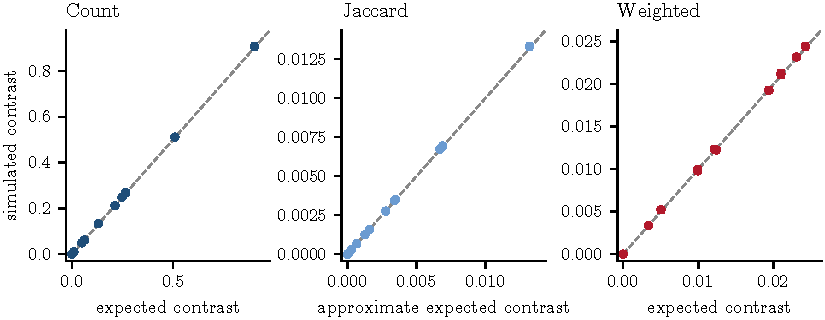
\includegraphics[width=\textwidth]{figA2_theory}
  \caption{Expected versus simulated within-minus-between contrast, one point per condition, with 95\% intervals. The dashed line marks equality. Each panel uses its own units; \Jac{} uses the ratio-of-expectations approximation.}
  \label{fig:theory}
\end{figure}

\section{Reproducibility}
\label{app:repro}

All simulations use Python 3.11 with the package versions recorded in \texttt{requirements-lock.txt}. Root seeds are 23601 (pilot), 23603 (main experiment), 23604 ($r=3$), 23605 (fixed-information experiment), 23607 ($r=4$), and 23606 (label permutations). Every data set's seed and $k$-means seed is stored, so any purchase matrix can be regenerated without storing it. Within each post hoc data set all methods share one $k$-means seed, which makes the exact equivalence of \Count{} and \Wtd{} under equal activity visible in the results. Unit tests check the design identities, label matching, recovery of a known partition, and the theoretical moments against simulation; validation scripts check every saved summary and paired interval. Mean runtimes per data set were 12.5\,ms for \Count, 12.8\,ms for \Jac, 14.8\,ms for \Wtd, and 48.2\,ms for \SVD, excluding data generation. The repository, \url{https://github.com/diaomj668/236project}, lists the commands that reproduce every result and figure in this report.

\section{Complete results}
\label{app:tables}

\begin{figure}[H]
  \centering
  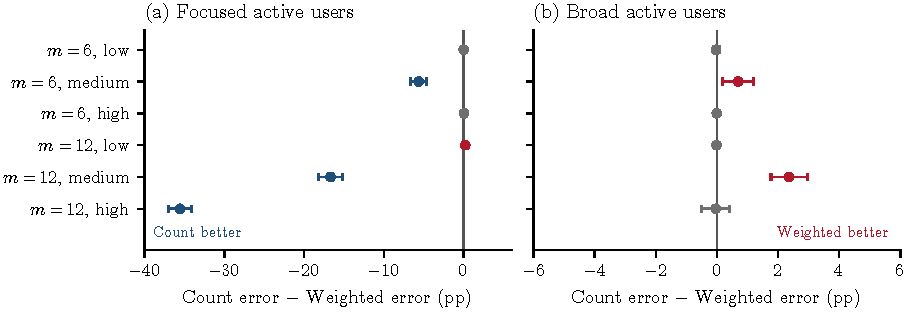
\includegraphics[width=\textwidth]{fig4_paired}
  \caption{Paired difference in misclustering rate, \Count{} minus \Wtd, with 95\% intervals over 100 data sets. Negative values favour \Count. Note the different horizontal scales.}
  \label{fig:paired}
\end{figure}

\begin{figure}[H]
  \centering
  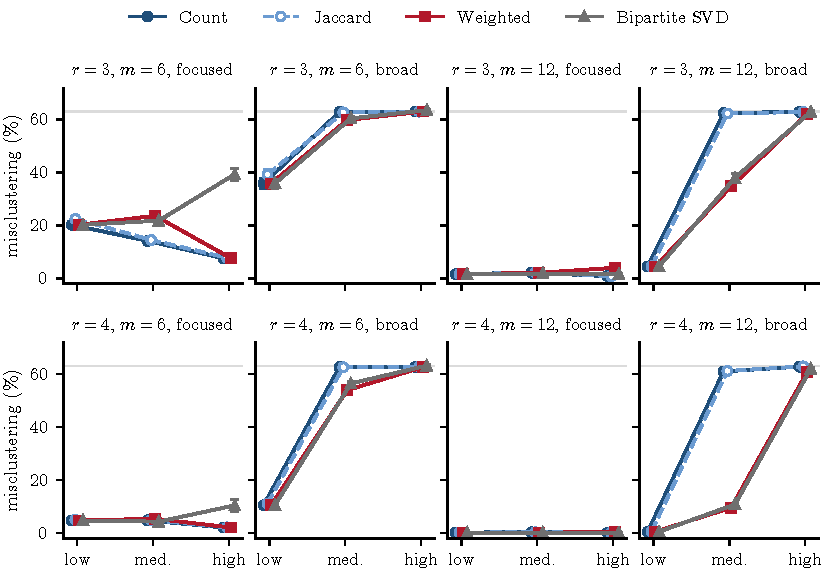
\includegraphics[width=\textwidth]{figA1_strength_grids}
  \caption{Post hoc sensitivity analyses at $r=3$ (top) and $r=4$ (bottom), with the same layout as \cref{fig:recovery}. The grey band marks the random-label reference.}
  \label{fig:grids}
\end{figure}

\begin{table}[H]
\centering\small
\caption{Results at $r=2$: mean misclustering rate (\%) over 100 data sets per condition.}
\label{tab:main}
\begin{tabular}{@{}cllcccc@{}}
\toprule
$m$ & Heterogeneity & Active users & \textsc{Count} & \textsc{Jaccard} & \textsc{Weighted} & \textsc{SVD} \\
\midrule
6 & low & focused & 59.8 & 59.9 & 59.8 & 59.8 \\
6 & low & broad & 60.5 & 60.8 & 60.6 & 60.5 \\
6 & medium & focused & 53.2 & 53.9 & 58.8 & 58.8 \\
6 & medium & broad & 62.8 & 62.9 & 62.1 & 62.6 \\
6 & high & focused & 41.3 & 42.3 & 41.2 & 59.7 \\
6 & high & broad & 62.9 & 62.6 & 62.9 & 63.2 \\
\addlinespace
12 & low & focused & 35.5 & 36.3 & 35.3 & 35.5 \\
12 & low & broad & 48.5 & 49.2 & 48.5 & 48.5 \\
12 & medium & focused & 22.4 & 22.7 & 39.0 & 37.0 \\
12 & medium & broad & 62.6 & 62.8 & 60.2 & 60.3 \\
12 & high & focused & 13.0 & 13.1 & 48.6 & 47.8 \\
12 & high & broad & 62.9 & 62.9 & 63.0 & 63.2 \\
\bottomrule
\end{tabular}
\end{table}
\begin{table}[H]
\centering\small
\caption{Results at $r=3$: mean misclustering rate (\%).}
\label{tab:r3}
\begin{tabular}{@{}cllcccc@{}}
\toprule
$m$ & Heterogeneity & Active users & \textsc{Count} & \textsc{Jaccard} & \textsc{Weighted} & \textsc{SVD} \\
\midrule
6 & low & focused & 20.2 & 22.5 & 20.2 & 20.2 \\
6 & low & broad & 35.9 & 39.2 & 35.9 & 35.9 \\
6 & medium & focused & 14.2 & 14.5 & 23.7 & 21.8 \\
6 & medium & broad & 62.9 & 62.7 & 59.8 & 60.5 \\
6 & high & focused & 7.6 & 7.8 & 7.6 & 39.3 \\
6 & high & broad & 63.1 & 63.0 & 63.1 & 63.5 \\
\addlinespace
12 & low & focused & 1.6 & 1.6 & 1.6 & 1.6 \\
12 & low & broad & 4.5 & 4.6 & 4.5 & 4.5 \\
12 & medium & focused & 2.1 & 2.2 & 2.1 & 1.8 \\
12 & medium & broad & 62.5 & 62.3 & 34.8 & 38.0 \\
12 & high & focused & 0.9 & 0.9 & 4.0 & 1.6 \\
12 & high & broad & 62.9 & 62.9 & 62.2 & 63.0 \\
\bottomrule
\end{tabular}
\end{table}
\begin{table}[H]
\centering\small
\caption{Results at $r=4$: mean misclustering rate (\%).}
\label{tab:r4}
\begin{tabular}{@{}cllcccc@{}}
\toprule
$m$ & Heterogeneity & Active users & \textsc{Count} & \textsc{Jaccard} & \textsc{Weighted} & \textsc{SVD} \\
\midrule
6 & low & focused & 4.7 & 5.0 & 4.7 & 4.7 \\
6 & low & broad & 10.5 & 11.0 & 10.5 & 10.5 \\
6 & medium & focused & 4.8 & 4.9 & 5.4 & 4.3 \\
6 & medium & broad & 62.7 & 62.6 & 53.9 & 56.5 \\
6 & high & focused & 2.1 & 2.1 & 2.1 & 10.4 \\
6 & high & broad & 62.7 & 62.9 & 62.7 & 63.2 \\
\addlinespace
12 & low & focused & 0.1 & 0.1 & 0.1 & 0.1 \\
12 & low & broad & 0.5 & 0.5 & 0.5 & 0.5 \\
12 & medium & focused & 0.3 & 0.3 & 0.1 & 0.1 \\
12 & medium & broad & 61.0 & 61.2 & 9.6 & 10.8 \\
12 & high & focused & 0.1 & 0.1 & 0.3 & 0.1 \\
12 & high & broad & 62.9 & 62.9 & 60.7 & 62.1 \\
\bottomrule
\end{tabular}
\end{table}
\begin{table}[H]
\centering\small
\caption{Fixed-information experiment: mean misclustering rate (\%) over 100 data sets. $A$ is the number of added preference-free users and $D/m$ their purchases relative to the informative users.}
\label{tab:separation}
\begin{tabular}{@{}lcccccc@{}}
\toprule
Informative users & $A$ & $D/m$ & \textsc{Count} & \textsc{Jaccard} & \textsc{Weighted} & \textsc{SVD} \\
\midrule
$m=12$, $r=2$ & 0 & -- & 35.5 & 36.4 & 35.5 & 35.5 \\
 & 50 & 1 & 37.1 & 37.4 & 37.1 & 37.1 \\
 & 50 & 2 & 45.9 & 46.3 & 36.6 & 36.8 \\
 & 50 & 4 & 59.0 & 59.2 & 36.0 & 36.3 \\
 & 50 & 8 & 61.7 & 61.8 & 35.7 & 36.1 \\
 & 200 & 1 & 40.7 & 41.5 & 40.7 & 40.7 \\
 & 200 & 2 & 54.9 & 55.2 & 40.2 & 40.3 \\
 & 200 & 4 & 61.5 & 61.4 & 39.3 & 39.8 \\
 & 200 & 8 & 62.0 & 62.0 & 36.9 & 38.3 \\
\addlinespace
$m=6$, $r=3$ & 0 & -- & 20.5 & 22.3 & 20.5 & 20.5 \\
 & 50 & 1 & 21.8 & 23.5 & 21.8 & 21.8 \\
 & 50 & 2 & 31.7 & 34.4 & 21.5 & 21.8 \\
 & 50 & 4 & 56.8 & 57.3 & 21.6 & 22.3 \\
 & 50 & 8 & 61.4 & 61.6 & 21.4 & 22.7 \\
 & 200 & 1 & 25.4 & 27.3 & 25.4 & 25.4 \\
 & 200 & 2 & 49.2 & 50.2 & 24.8 & 26.2 \\
 & 200 & 4 & 61.0 & 60.9 & 24.5 & 27.0 \\
 & 200 & 8 & 62.3 & 62.4 & 23.5 & 26.4 \\
\bottomrule
\end{tabular}
\end{table}


\end{document}
